% IOP Publishing journal article prepared from manuscript/main/quantum-template.tex
\documentclass{iopjournal}

\usepackage[utf8]{inputenc}
\usepackage[english]{babel}
\usepackage[T1]{fontenc}
\usepackage{amsmath,amssymb,amsfonts}
\usepackage{amsthm}
\usepackage{mathrsfs}
\usepackage{booktabs}
\usepackage{array}
\usepackage{multirow}
\usepackage{textcomp}
\usepackage{placeins}
\usepackage{xurl}

\newtheorem{theorem}{Theorem}

\begin{document}

\articletype{Paper}

\title{Risk-Aware Template-Switching Control under Partial Quantum Observability}

%\author{Jaeyun Jeong$^1$\orcid{0009-0005-3281-5858} and Hwa Young Jeong$^2$\orcid{0000-0002-5017-934X}}

%\affil{$^1$Division of Computer Engineering, Hankuk University of Foreign Studies, 17035 Yongin, Republic of Korea}

%\affil{$^2$Humanitas College, Kyung Hee University, 26, Kyungheedae-ro, 02447 Seoul, Republic of Korea}

%\email{3500jjy@gmail.com; hyjeong@khu.ac.kr}

\keywords{template switching; partial observability; finite-clock model; state restoration; quantum information; risk-aware control}

\begin{abstract}
Quantum decision rules under partial observability can make harmful switches to a
discrete reference template even when the template fits the available data.  We
study whether an observable veto can identify such switches without using the
hidden target state.  An audit of our originally submitted three-qubit
simulations found a degenerate clock-conditioned representation and a veto
effect driven solely by an additive uncertainty threshold.  Those submitted-grid
results are consequently retained only as an audit, not as evidence for a
relational-spectral advantage.  R1 supplies a finite, energy-matched
clock--logical-system qualification.  R3 then compares a continuous estimate,
a direct nearest-template estimate, score-only, uncertainty-only, and a
corrected held-out residual gate: both candidates are fitted on four clock labels
and scored unchanged on the complementary four labels.  Across four frozen
stream families with disjoint bank/calibration/test partitions, the residual gate reduces the harmful
template-switch rate relative to score-only in every evaluated grid cell.  Its
combined uncertainty-plus-residual form has no uniform advantage over the
uncertainty gate, and its mean-fidelity difference relative to the continuous
estimate is not consistently positive.  The supported contribution is therefore
a bounded template-switching safety analysis under a known finite-clock model,
not a generic QEC decoder, an unknown-state recovery channel, or a performance
advantage attributable to a spectral representation.
\end{abstract}

%% ============================================================
%% REVISED INTRODUCTION
%% Target: IOP Quantum Science and Technology
%% Strategy: engineering/control framing first;
%%           relational dynamics demoted to motivation source;
%%           C3R contribution and downside-risk improvement
%%           foregrounded; claim boundary sharpened throughout.
%% ============================================================

\section{Introduction}\label{sec:introduction}

Quantum recovery increasingly has to operate under incomplete and
imperfect diagnostic information. In encoded quantum systems, syndrome
measurements provide the primary evidence for selecting a correction,
but this evidence may be missing, corrupted, ambiguous, or affected by
measurement and reset errors. Standard recovery and mitigation
frameworks address important aspects of this problem through recovery
maps, syndrome-based correction, autonomous protection, probabilistic
cancellation, and learning-based error
mitigation~\cite{Lautenbacher2024PetzRecoveryQudit,Gertler2021AutonomousQECBosonic,VanDenBerg2023SparsePauliLindbladPEC,Strikis2021LearningBasedQEM,Liao2024MachineLearningQEM}.
However, when observability is partial, mean fidelity improvement is
an insufficient criterion. A recovery policy may improve the average
logical fidelity while still producing rare but severe lower-tail
failures: a proposed correction that the degraded syndrome evidence
appeared to support turns out to worsen the protected state. These
unsafe candidate switches are the central failure mode this work
targets. An intervention mechanism that can selectively identify and
veto unsafe proposed switches---without disrupting reliable recovery
under adequate syndrome evidence---would provide a conservative
safety layer above syndrome-first recovery pipelines.

The submitted work proposed to construct such an intervention signal from
clock-conditioned graph spectra.  The audit reported here shows that this
submitted construction does not identify a relational-spectral gate: its
conditional density is constant and its admissibility condition is nonbinding.
We retain the construction only to document that failure mode.  The replacement
experiments use an energy-matched finite clock and observed count records; the
decision gate is stated directly as a held-out residual condition rather than as
a claim about relational spectral evidence.

Graph and spectral representations remain useful descriptive tools for the
submitted audit~\cite{Braunstein2006GraphLaplacianDensityMatrix,Adhikari2017WeightedDigraphsQuantumStates,Biamonte2019ComplexNetworksQuantum}.
They are not, however, the active evidence source for the revised safety claim.
R3 uses the same finite-clock labels to create a fitting/validation split and
asks the simpler operational question of whether a fixed template predicts the
withheld count records as well as the continuous candidate.

The revised study instead addresses a decision-control question that is common
to finite-data restoration: when a discrete template and a continuous estimate
are both available, can held-out observations identify template switches that
are likely to be harmful?  This is complementary to characterization and
uncertainty-quantification methods for finite observations
\cite{Hashim2025BenchmarkingCharacterization,Cieslinski2024RandomisedMeasurements,Bennink2026UncertaintyQuantificationQC},
but it is not a claim that this controller replaces a syndrome decoder or a
channel-level mitigation method.

R3 evaluates this question in a controlled encoded logical-qubit testbed.
Candidate \(A\) is a continuous Bloch-ball projected least-squares estimate and
candidate \(B\) is the direct nearest template under the same fitting-label
loss.  A policy may accept or veto a proposed switch from \(A\) to \(B\).  The
held-out gate can only veto a proposal; it cannot create a template switch.  The
comparison therefore exposes both harmful-switch reduction and any loss of mean
fidelity relative to the continuous candidate.

This revision takes a different evidentiary path.  An audit found that the
submitted clock construction has a constant conditional system state and that
its apparent veto effect disappears when the uncertainty threshold is removed.
The submitted stress-grid tables are therefore retained only as a transparent
historical audit; they do not establish relational-spectral recovery efficacy.

The revised contribution is a constrained risk-control test.  R1 supplies an
explicit, energy-matched finite-clock construction with nonconstant conditional
states.  R3 supplies four disjoint bank/calibration/test streams, physical code
noise, direct-template and uncertainty-only controls, a corrected held-out
residual gate, and two-way target-pair/measurement-seed intervals.  The residual
gate reduces harmful template switches relative to score-only selection in every
evaluated cell of every stream.  Its combined uncertainty-plus-residual version
does not have a uniform advantage over uncertainty-only selection, and it does
not establish a mean-fidelity advantage over the continuous estimate.

\section{Background and Positioning}
\subsection{Clock-conditioned relational dynamics}

Relational formulations of quantum dynamics describe change through correlations
with an internal clock rather than an externally supplied time parameter. This
idea appears in background-independence and relational-dynamics
discussions~\cite{Smolin2005BackgroundIndependence,Rovelli2007QuantumGravity}.
The Page--Wootters mechanism gives the operational ingredient used here: a
constrained global state can be conditioned on a clock subsystem to obtain
relative system states~\cite{Giovannetti2015QuantumTime,Marletto2017EvolutionWithoutEvolution,Hoehn2021TrinityRelationalQuantumDynamics}.
Related work has studied robustness, interactions, noncausal circuits,
measurement-related time flow, and computational uses of quantum
time~\cite{Rijavec2023RobustnessPageWootters,Mendes2021NonlinearPageWootters,Baumann2022NoncausalPageWoottersCircuits,Paiva2022FlowTimeEnergyMeasurements,Diaz2025ParallelPageWoottersSimulation}.
Our use of this literature is intentionally narrow. We do not attempt to solve
the problem of time or derive continuum dynamics from a finite clock; we use
clock-conditioned slices as finite relational data objects for recovery control.

\subsection{Spectral graph representations of quantum structure}

Graph-based and spectral representations provide compact descriptions of relational 
structure. In quantum information, graph Laplacians have been related to density matrices, 
separability, and quantum-state representations~\cite{Braunstein2006GraphLaplacianDensityMatrix,Adhikari2017WeightedDigraphsQuantumStates,Bradshaw2023GraphZetaEntanglement}. 
More broadly, quantum network models provide a language for connecting graph structure, 
correlations, and quantum dynamics~\cite{Biamonte2019ComplexNetworksQuantum}. These works 
motivate the use of spectral signatures as auditable summaries of relational connectivity.

The submitted work differed from graph-state or network modeling approaches in its
use of clock-conditioned spectral families. A single graph spectrum was not the
central object; each internal clock label produced a relational graph, and the
ordered family of Laplacian spectra defined a relational spectral trajectory.
The revision retains that construction only to make the failed submitted-grid
mechanism auditable. It is not an evidence source for R3.

\subsection{Quantum recovery, mitigation, and control}
Quantum recovery and error mitigation have developed along several complementary directions. 
Recovery-map approaches formalize channel-level reconstruction and approximate reversibility~\cite{Lautenbacher2024PetzRecoveryQudit}, 
while quantum error-correction experiments and autonomous protection schemes demonstrate 
how encoded or stabilized systems can preserve quantum information under noise~\cite{Reed2013EntanglementQEC,Gertler2021AutonomousQECBosonic,Nascimento2011NoiselessSubsystem}. In the NISQ setting, mitigation methods such as probabilistic error cancellation, virtual distillation, detection-based mitigation, and learning-based correction address noisy circuit outputs without requiring full fault tolerance~\cite{VanDenBerg2023SparsePauliLindbladPEC,Xu2024CircuitNoiseResilientVirtualDistillation,Zhang2021AutoencoderErrorMitigation,Strikis2021LearningBasedQEM,Liao2024MachineLearningQEM,Liao2025NoiseAgnosticQEM}.

The proposed framework is not a replacement for these methods. It is closer 
to a recovery-control layer placed above candidate recovery mechanisms. In the 
submitted encoded-QEC experiments, the syndrome-first recovery was the
decoder-facing baseline, while the relational admissible recovery supplied an
alternative candidate. The policy layer made a historical switch decision. R3
replaces this comparison with equal-information continuous and direct-template
candidates scored by a held-out count-record residual.

\subsection{Partial observability, uncertainty, and benchmarking}

Reliable recovery decisions depend on how much diagnostic information is available and 
how trustworthy that information is. Benchmarking and characterization methods provide 
tools for quantifying device behavior and validating performance claims~\cite{Hashim2025BenchmarkingCharacterization}. 
Randomized-measurement techniques and uncertainty-quantification frameworks also emphasize 
that finite, noisy, or incomplete observations must be interpreted with calibrated uncertainty~\cite{Cieslinski2024RandomisedMeasurements,Bennink2026UncertaintyQuantificationQC}. 
Noise modeling, live noise fingerprinting, robust control, and non-Markovian noise studies 
further show that quantum behavior can depend strongly on the structure and timing of noise 
processes~\cite{Ji2026DataEfficientNoiseModeling,Bensoussan2025LiveNoiseFingerprinting,Ding2025UniversallyRobustControl,Cai2020RandomTelegraphDephasing,Zhang2024NonMarkovianTeleportation,Zhuang2026FluxoniumNonMarkovian}.

The present study focuses on a narrower but related issue: unsafe candidate selection 
when syndrome evidence is partial or jointly corrupted. Rather than claiming a calibrated 
posterior uncertainty model, we use a deliberately simple syndrome-stress index and evaluate 
its behavior through threshold and uncertainty-bin diagnostics. This makes the controller 
auditable and exposes the tradeoff between preventing harmful switches and mistakenly 
blocking beneficial ones.

\section{Submitted framework and metrics (archival)}\label{sec:methods}

This section documents the framework used to generate the submitted grid so that
the audit is reproducible. It is not the primary method supporting the revised
claim. The audit in Section~\ref{sec:results} establishes that the instantiated
clock-conditioned trajectory is degenerate and that the submitted admissibility
gate is nonbinding. Accordingly, the relational-spectral construction, recovery
objective, and syndrome-stress policy below are historical implementation
specifications rather than validated ingredients of R3. The corrected R3 method
and the only positive efficacy evidence in this revision are given in
Section~\ref{sec:revision-results}. Figure~\ref{fig:pipeline-overview} therefore
summarizes the submitted pipeline, not a validated recovery procedure.

\begin{figure}[t]
\centering
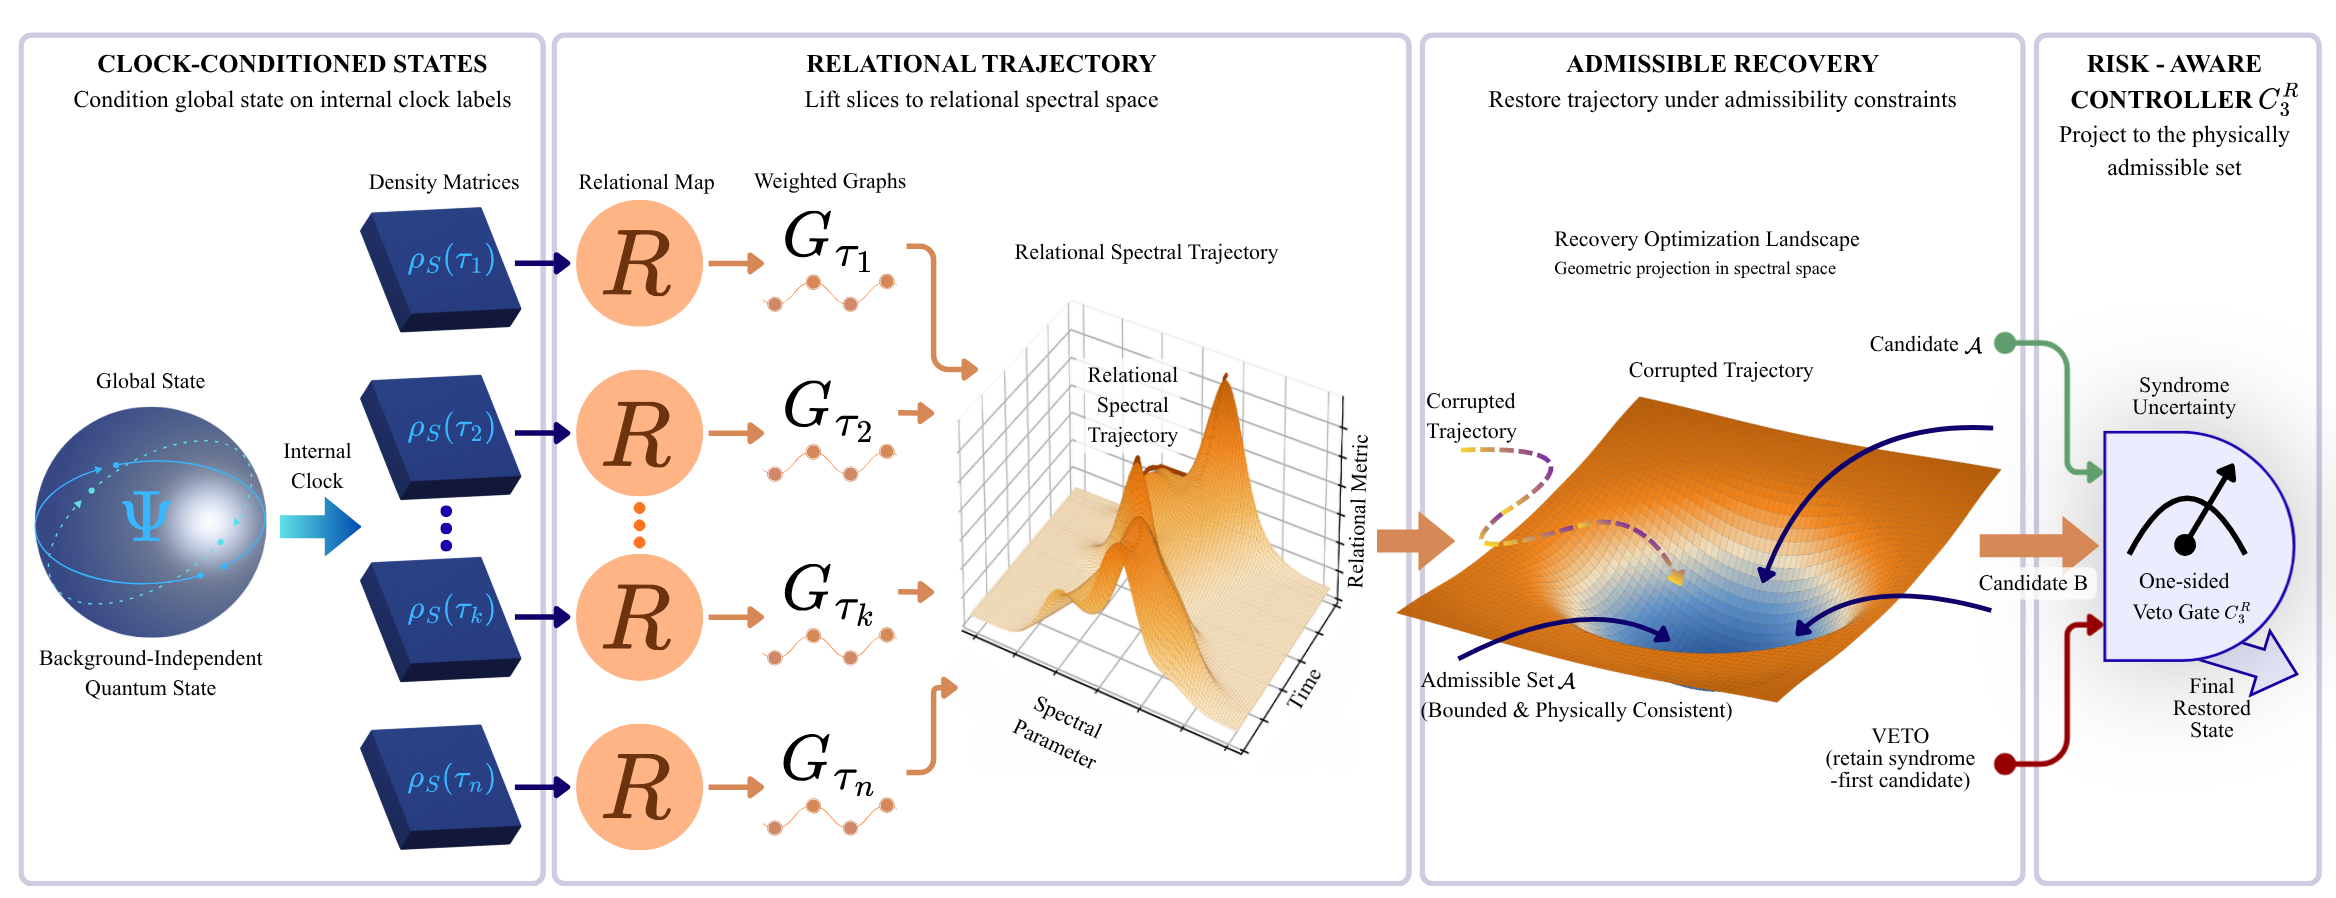
\includegraphics[width=0.95\textwidth]{main_figure.png}
\caption{Submitted-pipeline overview, retained for audit reproducibility.
A constrained global state is conditioned on internal clock labels to obtain system slices \(\rho_S(\tau_r)\).
Each slice is mapped to a weighted relational graph and reduced to a Laplacian spectral signature, yielding the relational spectral trajectory \(\Gamma_\Psi\).
The observed trajectory is restored through a reference-anchored admissible recovery objective, producing the relational candidate \(B\).
At the policy layer, \(C_3^R\) acts as a one-sided veto that can retain the syndrome-first candidate \(A\) or accept the \(C_2\)-proposed switch to \(B\).
The audit finds that this instantiated pipeline does not identify a
relational-spectral efficacy effect.
}
\label{fig:pipeline-overview}
\end{figure}

\subsection{Clock-conditioned relational formulation (submitted configuration)}
\label{subsec:relational-formulation}

The following formalism states the submitted intended construction. The audit
shows that its actual implementation, specified below with $H_S=0$, does not
satisfy the required nondegenerate conditional-trajectory premise; it is retained
only to define the historical artifact. We use a clock-conditioned relational
formulation inspired by
background-independent quantum dynamics and relational-time
constructions~\cite{Gambini2004RelationalTime,Giovannetti2015QuantumTime,Hoehn2021TrinityRelationalQuantumDynamics}.
The total Hilbert space is decomposed as
\begin{equation}
\mathcal{H}_{\mathrm{tot}}
=
\mathcal{H}_{C}\otimes\mathcal{H}_{S},
\end{equation}
where $\mathcal{H}_{C}$ is an internal clock register and $\mathcal{H}_{S}$ is the
system register. Rather than assuming an externally supplied time coordinate, we
work with a constrained global state
\begin{equation}
\hat{H}_{\mathrm{tot}}|\Psi\rangle=0.
\end{equation}
We use this global constraint not as a claim that the finite simulation realizes a
complete Wheeler--DeWitt theory or quantum-cosmological
dynamics~\cite{Mazzitelli1992Midisuperspace,Massar1999UnitaryNonunitaryEvolution,Maki2026WheelerDeWittSolutions},
but as a construction principle for generating internally indexed conditional
system slices. In the computational pipeline, the
role of the constraint is to define the admissible clock-conditioned family
$\{\rho_S(\tau_r)\}_{r=1}^{m}$, from which all relational spectra, recovery
objectives, and policy diagnostics are derived. In a finite-dimensional
simulation, the existence and resolution of clock labels depend on spectral
matching and recurrence constraints; those conditions are treated as consistency
requirements and are moved to the Supplementary Information.

For a clock label $\tau$, the clock-conditioned system state is
\begin{equation}
\rho_S(\tau)
=
\frac{
\operatorname{Tr}_{C}\!\left[
\left(|\tau\rangle\langle\tau|_{C}\otimes I_S\right)
|\Psi\rangle\langle\Psi|
\right]
}{
\operatorname{Tr}\!\left[
\left(|\tau\rangle\langle\tau|_{C}\otimes I_S\right)
|\Psi\rangle\langle\Psi|
\right]
}.
\label{eq:clock-conditioned-state}
\end{equation}
We therefore do not model recovery as a trajectory over an externally supplied
background time coordinate. Instead, we condition a timeless global state on
internal clock labels and construct recovery evidence from the resulting
relational slices. Detailed consistency conditions for the global constraint,
finite-dimensional clock representation, and clock-resolution assumptions are
provided in Supplementary Note S1.
In the implementation, each encoded simulation instance uses one clock qubit with
initial state $|+\rangle_C$ and clock Hamiltonian $H_C=0.8X_C$. The clock grid is
uniform with
\begin{equation}
m=9,\qquad
\tau_r\in\{-2.0,-1.5,\ldots,1.5,2.0\}.
\end{equation}
The conditional states $\rho_S(\tau_r)$ are materialized from the simulated global
density matrix using Eq.~\eqref{eq:clock-conditioned-state}. Unless otherwise
stated, the same clock grid, clock Hamiltonian, and conditional-slice construction
are used for all policies and stress protocols. This finite sampling is also why
the framework is naturally compatible with partial observability: a degraded
experiment may hide or corrupt part of the evidence available to the policy layer
without changing the underlying definition of a clock-conditioned slice.
The one-qubit clock is used deliberately as a minimal finite relational clock,
not as a continuum-clock
approximation~\cite{Foti2021ClassicalEquationsPageWootters,Rijavec2023RobustnessPageWootters}.
This choice keeps the validation focused
on the minimal controlled question: whether clock-conditioned relational spectra
can provide auditable recovery evidence before scaling to larger clock registers
or denser relational clocks.

\subsection{Relational spectral representation (submitted configuration)}
\label{subsec:spectral-representation}

For each clock-conditioned state $\rho_S(\tau)$, we build a weighted relational
network whose edge weights encode pairwise relational evidence between system
degrees of freedom,
\begin{equation}
\begin{aligned}
W^{(\tau)}_{ij}
&=
f(\rho_S(\tau);i,j),\\
W^{(\tau)}_{ij}
&=
W^{(\tau)}_{ji},
\qquad
W^{(\tau)}_{ij}\ge 0.
\end{aligned}
\end{equation}
The submitted-grid experiments used explicit pairwise functionals rather than leaving
$f$ unspecified. Let $\rho_{ij}^{(\tau)}$ be the two-qubit reduction of
$\rho_S(\tau)$ and let $\rho_i^{(\tau)}$ be the one-qubit reduction. For
phase-flip-code experiments we use the absolute two-qubit coherence score
\begin{equation}
W^{(\tau)}_{ij}
=
\sum_{a\ne b}
\left|(\rho_{ij}^{(\tau)})_{ab}\right|,
\qquad i\ne j,
\label{eq:coherence-weight-main}
\end{equation}
in the computational basis. For bit-flip-code experiments we use the von Neumann
mutual-information score
\begin{equation}
W^{(\tau)}_{ij}
=
S(\rho_i^{(\tau)})
+
S(\rho_j^{(\tau)})
-
S(\rho_{ij}^{(\tau)}),
\label{eq:mutual-info-weight-main}
\end{equation}
with negative numerical round-off clipped to zero. Alternative pairwise
functionals are possible and are treated as representation-robustness questions
for future work, but the submitted-grid policy comparisons use the fixed code-dependent
mapping above.
The two choices reflect the dominant relational signature of the corresponding
encoded basis. Phase-flip protection is sensitive to phase coherence, so the
computational-basis coherence functional directly measures off-diagonal
relational structure. Bit-flip protection is associated with population-basis
error structure, for which mutual information provides a basis-independent
pairwise dependence score. Because this choice can affect
sensitivity, we treat representation robustness as a limitation rather than
claiming uniqueness of the graph functional.
We use a graph Laplacian rather than raw edge weights because its
spectrum summarizes collective connectivity, is stable under node relabeling, and
allows perturbations to be compared through standard spectral
quantities~\cite{JiangSpectralGraphTheory,Braunstein2006GraphLaplacianDensityMatrix,Adhikari2017WeightedDigraphsQuantumStates}.

The corresponding degree matrix and graph Laplacian are
\begin{equation}
D^{(\tau)}_{ii}=\sum_{j\neq i} W^{(\tau)}_{ij},
\qquad
L(\tau)=D^{(\tau)}-W^{(\tau)}.
\end{equation}
Let the ordered Laplacian spectrum be
\begin{equation}
\begin{aligned}
\Lambda(\tau)
&=
\left(\lambda_1(\tau),\ldots,\lambda_n(\tau)\right),\\
\lambda_1(\tau)
&\le
\cdots
\le
\lambda_n(\tau).
\end{aligned}
\end{equation}
The central object is not an individual graph or a single spectrum, but the
clock-conditioned spectral family
\begin{equation}
\Gamma_\Psi:T\rightarrow\mathbb{R}^{n},
\qquad
\Gamma_\Psi(\tau)=\Lambda(\tau).
\label{eq:spectral-family}
\end{equation}
We use the term trajectory to denote an ordered family over internal clock labels,
not evolution with respect to external background time.
This distinction matters for the recovery task. A local perturbation at one clock
slice may be harmless if it is compatible with the neighboring slices, but the same
perturbation can be suspicious if it creates a discontinuity in the spectral
family. The object being recovered is therefore the whole clock-indexed spectral
signature, not a collection of independent spectra. This representation is
intended to expose relational inconsistencies that may not be captured by a single
syndrome snapshot.

Computationally, the collection of admissible spectral families is treated as a
finite metric trajectory representation. For two spectral families
$\Gamma^{(a)}$ and $\Gamma^{(b)}$ sampled at clock labels
$\{\tau_r\}_{r=1}^{m}$, we use
\begin{equation}
\begin{aligned}
d_{\mathcal M}^{ab}
&\equiv
d_{\mathcal{M}}\!\left(\Gamma^{(a)},\Gamma^{(b)}\right),\\
d_{\mathcal M}^{ab}
&=
\left(
\sum_{r=1}^{m}
w_r
\left\|
\Lambda^{(a)}(\tau_r)-\Lambda^{(b)}(\tau_r)
\right\|_2^2
\right)^{1/2}.
\end{aligned}
\label{eq:trajectory-distance}
\end{equation}
The geometric terminology used below should be read as a formal interpretation of this finite metric trajectory representation. The detailed tangent-space,
geodesic, and perturbation arguments are given in Supplementary Notes S2 and S3.
The weights $w_r$ allow the implementation to emphasize or de-emphasize particular
clock slices, but the experiments reported here use the same metric form across
all policies. Thus differences between $C_1$, $C_2$, $C_3$, and
$C_3^{\mathrm R}$ arise from the decision layer, not from changing the underlying
trajectory distance.

\subsection{Admissible spectral recovery (submitted configuration)}
\label{subsec:admissible-recovery}

Let $\Gamma_{\mathrm{obs}}$ be the observed spectral trajectory after noise or
partial observation. Recovery is posed as a constrained restoration problem in
spectral-trajectory space. We define an admissible set
\begin{equation}
\mathcal{A}
=
\mathcal{A}_{\mathrm{lap}}
\cap
\mathcal{A}_{\mathrm{rel}}
\cap
\mathcal{A}_{\mathrm{ref}},
\end{equation}
where $\mathcal{A}_{\mathrm{lap}}$ enforces Laplacian spectral constraints,
$\mathcal{A}_{\mathrm{rel}}$ enforces relational smoothness and clock consistency,
and $\mathcal{A}_{\mathrm{ref}}$ constrains compatibility with a reference family.
In implementation these constraints are audited through penalty functions
$\{\Phi_k\}_{k\in\mathcal{K}}$ with calibrated thresholds $\{\theta_k\}$.
These three constraint classes play different roles. Laplacian constraints prevent
spectral objects that cannot arise from an admissible relational graph. Relational
smoothness penalizes abrupt clock-slice variation that is not supported by the
reference dynamics. Reference compatibility prevents the recovery from drifting
toward a structurally valid but physically irrelevant spectral family. We keep
these as separate penalties rather than collapsing them into a single score so
that later policy decisions can identify whether a candidate failed because of
structure, relational continuity, or reference mismatch.

In the experiments, $\Phi_{\mathrm{lap}}$ is the sum over clock slices of
structural Laplacian violations: symmetry error, positive-semidefinite violation,
row-sum violation, positive off-diagonal violation, and diagonal-consistency
error. $\Phi_{\mathrm{smooth}}$ penalizes slice-to-slice spectral jumps by summing
$\|\Lambda(\tau_{r+1})-\Lambda(\tau_r)\|_2^2/(\tau_{r+1}-\tau_r)^2$.
$\Phi_{\mathrm{clock}}$ compares spectral response between neighboring slices to
the distinguishability of the corresponding clock states, and
$\Phi_{\mathrm{ref}}$ is the squared distance to the nearest reference trajectory.
In the submitted implementation, thresholds were calibrated as
$\mu+\kappa\sigma$ over the reference bank, with $\kappa=1.5$. The associated
calibration sweep is retained in the SI as historical implementation detail; it
does not establish a discriminative admissibility gate on the submitted grid.

For a candidate trajectory $\Gamma_X$, the normalized admissibility violation is
\begin{equation}
v_X
:=
\max_{k\in\mathcal{K}}
\max\left\{0,
\frac{\Phi_k(\Gamma_X)-\theta_k}{\theta_k+\epsilon}
\right\}.
\label{eq:normalized-violation-main}
\end{equation}
Thus $v_X=0$ means that all active constraints are within threshold, while
positive values measure the worst normalized excursion beyond the admissible
boundary.

Admissibility defines which spectral families are physically and structurally
acceptable. It does not by itself provide a restoration direction. We therefore
introduce a reference-anchor term that explicitly pulls the recovered trajectory
toward the nearest compatible reference family. Given a reference bank
$\mathcal{R}$, the anchor is
\begin{equation}
\Gamma_{\mathrm{ref,anchor}}
=
\arg\min_{\Gamma'\in\mathcal{R}}
d_{\mathcal{M}}\!\left(\Gamma',\Gamma_{\mathrm{obs}}\right)^2.
\end{equation}
This anchor is the key distinction between feasibility and recovery. A projection
onto $\mathcal{A}$ alone could return a trajectory that is merely allowed; it need
not be the trajectory most compatible with the unperturbed relational behavior.
The reference bank supplies a local restoration direction without requiring the
method to know the clean trajectory of the test instance. In the encoded
experiments, the bank contains three clean reference trajectories per code
configuration: the corresponding logical reference state for the code
configuration and two phase-rotated logical references at $\pm20^\circ$. The bank
is generated with the same code, clock grid, clock Hamiltonian, and graph
functional as the test row, but with the noise schedule removed. For each
observed trajectory, the anchor is selected using
only $d_{\mathcal M}(\Gamma',\Gamma_{\mathrm{obs}})$; no clean logical outcome,
candidate fidelity, or row-level oracle information is used during anchor
selection.
The three-anchor bank is intentionally minimal. It tests whether a small
auditable reference family can support recovery-side control, not whether a dense
clean-state manifold has been approximated.

The recovery objective is
\begin{equation}
\begin{aligned}
J_{\mathrm{rec}}(\Gamma)
= {}&
\alpha
d_{\mathcal{M}}\!\left(\Gamma,\Gamma_{\mathrm{obs}}\right)^2
\\
&+
\beta
d_{\mathcal{M}}\!\left(\Gamma,\Gamma_{\mathrm{ref,anchor}}\right)^2
\\
&+
\lambda_1\Phi_{\mathrm{lap}}(\Gamma)
+
\lambda_2\Phi_{\mathrm{smooth}}(\Gamma)
\\
&+
\lambda_3\Phi_{\mathrm{clock}}(\Gamma).
\end{aligned}
\label{eq:recovery-objective-main}
\end{equation}
The first term keeps the recovered trajectory close to the observation, so the
method does not discard the measured evidence. The second term pulls the solution
toward the nearest compatible reference family, providing the actual restoration
direction. The penalty terms then audit whether the resulting trajectory remains
structurally and relationally admissible. This separation is deliberate: a
candidate can be close to the observation but inadmissible, admissible but pointed
toward the wrong reference family, or reference-compatible but too discontinuous
across clock labels.

In the submitted-grid experiments, we use the discrete admissible projection as the default
recovery operator because it is stable, interpretable, and directly auditable.
Continuous convex refinement is treated as a diagnostic extension and reported in
the Supplementary Information. Further details on admissibility penalties,
reference-bank construction, anchor-weight calibration, and the two-stage recovery
algorithm are provided in Supplementary Note S4.

\subsection{Encoded-QEC protocol (submitted grid only)}\label{subsec:qec-validation}

Revision status: the configuration described in this subsection is the submitted
grid, retained to make the audit reproducible.  It has a degenerate conditional
clock trajectory and cannot support an efficacy claim; its reported quantities
are consequently labelled historical.  The nondegenerate finite-clock check and
the held-out switching experiment that support the revised scope are reported in
Section~\ref{sec:revision-results} and in the supplementary section ``Revision
audit and new experiments.''

The submitted encoded-QEC setting was designed as a controlled testbed for partial
observability and unsafe recovery transitions. It does not support a decoder claim:
the audit shows that its relational evidence is degenerate and its admissibility
gate is inactive. The details below describe how complete, missing, corrupted,
ambiguous, measurement-, and reset-error syndrome conditions were generated for
the historical audit. R3 instead tests a two-candidate count-record decision
problem with equal-information candidates.

Each submitted-grid simulation row produced two candidates:
\begin{equation}
A := \text{syndrome-first decoded recovery},
\qquad
B := \text{relational admissible recovery}.
\end{equation}
Candidate $A$ was obtained by applying the code-specific syndrome recovery rule to
the underlying noisy density. Candidate $B$ was obtained by the admissible
spectral recovery objective in Eq.~\eqref{eq:recovery-objective-main}. The policy
then made the historical switch decision. As detailed in the SI, degraded syndrome
symbols affected controller support rather than the candidate-$A$ recovery
channel.
Both candidates are evaluated against the same clean logical trajectory when
computing outcomes, but the policy layer does not use that clean trajectory when
making the decision. It sees only the candidate diagnostics, observed syndrome
summary, admissibility reports, recovery objective, and uncertainty proxy. This
separation is necessary because the intervention metrics later use the clean
trajectory only as offline ground truth for analysis.

The submitted-grid experiments use three-qubit repetition codes in bit-flip and phase-flip
configurations, with bit-flip, phase-flip, depolarizing, dephasing, and mixed-Pauli
noise families. Each reported regime cell is averaged over seeds $11$--$20$,
giving ten random seeds per cell. The output-stem suffix \texttt{seed10} is a
batch label for this ten-seed set. The encoding and syndrome-extraction circuits
for both code configurations are shown in Supplementary Figs.~S1 and~S2.
Syndrome observability is controlled by the observation ratio
$r_{\mathrm{obs}}$, syndrome-bit corruption probability $p_{\mathrm{noise}}$,
ambiguity level $a_{\mathrm{amb}}$, measurement error probability $p_{\mathrm{meas}}$,
reset error probability $p_{\mathrm{reset}}$, and measured syndrome information loss
$\ell_{\mathrm{syn}}$. These quantities define the raw and clipped uncertainty
proxies
\begin{equation}
u_{\mathrm{raw}}
=
(1-r_{\mathrm{obs}})
+p_{\mathrm{noise}}
+a_{\mathrm{amb}}
+p_{\mathrm{meas}}
+p_{\mathrm{reset}}
+\ell_{\mathrm{syn}},
\qquad
u_{\mathrm{syn}}=\mathrm{clip}_{[0,1]}(u_{\mathrm{raw}}).
\end{equation}
The uncertainty proxy is a deliberately simple additive stress index rather than a
calibrated posterior uncertainty. The clipped value is used by the decision gate
so that $u_{\max}=0.99$ implements a conservative saturation rule: saturated
uncertainty blocks a proposed relational switch, while non-saturated uncertainty
leaves the $C_2$ proposal eligible. The raw uncertainty is retained for diagnostics
and bin-wise analysis. This distinction is important in the partial-plus-noisy and
ambiguity-plus-measurement regimes, where several moderate degradations can combine
into saturated decision uncertainty.

We compare four policies on the same candidates $A$ and $B$. $C_1$ is a
rule-based conservative hybrid that switches to $B$ only when $A$ is inadmissible
and $B$ is admissible, or when $B$ is admissible, has lower recovery objective, and
the observed syndrome is consistent. $C_2$ is the balanced proposal policy
\begin{equation}
S_X^{(2)}
=
\lambda_s s_X
-\lambda_t d_X
-\lambda_i(1-a_X)
+\lambda_o\frac{1}{1+J_X},
\end{equation}
where $a_X$ is the admissibility indicator, $d_X$ is the trajectory distance to the
observed trajectory, and $s_X$ is the syndrome-support score. The current
experiments use
\begin{equation}
(\lambda_s,\lambda_t,\lambda_i,\lambda_o)=(1.0,1.0,2.0,0.5).
\end{equation}
$C_3$ is a hard-admissibility ablation: if exactly one of $A$ and $B$ is
admissible, it selects the admissible candidate; otherwise it falls back to a
safety-weighted score. The initial $C_3$ policy was designed to test whether a
globally strict safety-first region exists. Because this strict policy did not form
an independent operating zone in the regime map, we use $C_3^{\mathrm{R}}$ as the
revised risk-aware controller that preserves the safety motivation of $C_3$ while
applying intervention only to proposed $C_2$ switches.
This submitted policy sequence is intentionally cumulative. $C_1$ represents a conservative
rule-based baseline. $C_2$ asks whether a balanced score can use relational
evidence without excessive switching. $C_3$ tests whether a strict Boolean
admissibility rule creates a distinct safety-first region. $C_3^{\mathrm R}$ is
the submitted controller: it keeps $C_2$ as the proposal
mechanism, but only allows its proposed switch to survive if additional safety and
uncertainty gates pass.

The robust policy $C_3^{\mathrm{R}}$ treats $C_2$ as a proposal and applies a
one-sided veto. Let $\Delta S=S_B^{(2)}-S_A^{(2)}$. The gate is
\begin{equation}
\begin{aligned}
C_3^{\mathrm{R}}=B
\Longleftrightarrow\;&
\left[C_2=B\right]
\\
&\wedge
\left[\Delta S\ge\delta_S\right]
\\
&\wedge
\left[v_A\ge\delta_A\right]
\\
&\wedge
\left[B\ \mathrm{admissible}\right]
\\
&\wedge
\left[v_B\le\delta_B\right]
\\
&\wedge
\left[u_{\mathrm{syn}}\le u_{\max}\right].
\end{aligned}
\label{eq:c3r-gate-main}
\end{equation}
Otherwise $C_3^{\mathrm{R}}=A$. The main operating point is
\begin{equation}
\begin{aligned}
\delta_S&=0,
\qquad
\delta_A=0,\\
\delta_B&=0,
\qquad
u_{\max}=0.99.
\end{aligned}
\end{equation}
Thus $C_3^{\mathrm{R}}$ can only block $C_2$ switches; it never creates additional
switches that $C_2$ rejected. The policy should therefore be interpreted as a
downside-risk controller rather than a fourth independently tuned score rule.
At the main operating point, the $v_A\ge\delta_A$ condition is nonrestrictive
because $v_A\ge0$ by definition. The active default gate therefore tests whether
the $C_2$-proposed relational candidate is score-supported, exactly admissible
within the calibrated tolerances, and not exposed to saturated syndrome
uncertainty. We keep the $v_A$ term in Eq.~\eqref{eq:c3r-gate-main} because it is
part of the general gate family and can be activated in ablations.
At this operating point, the uncertainty gate is the dominant veto mechanism in
saturated-stress rows, while the exact-admissibility condition prevents accepting
relational candidates that already violate the calibrated admissible set.
Complete policy maps, decision reasons, and operating-zone summaries are provided in
Supplementary Notes S5 and S6.
The clean-regime role of $C_3^{\mathrm R}$ is correspondingly limited. If syndrome
evidence is reliable and the uncertainty gate is open, the robust policy should
often reduce to $C_2$. Its value is tested primarily in regimes where syndrome
evidence is partial, corrupted, or ambiguous enough that a proposed relational
switch carries elevated downside risk.

\subsection{Evaluation metrics and operating criteria}\label{subsec:evaluation-metrics}

Since the controller is designed to suppress unsafe recovery transitions rather than
maximize average fidelity alone, we evaluate both central performance and
lower-tail risk. For each policy $C$, let
\begin{equation}
\Delta F_C=F_C-F_{\mathrm{before}}
\end{equation}
be the logical-fidelity gain relative to the noisy observed trajectory before
recovery. Central performance is summarized by the mean gain
$\overline{\Delta F}_C$, the logical-success rate
$P(F_C\ge F_{\mathrm{success}})$, and the non-worsening rate
$P(\Delta F_C\ge0)$.
Unless otherwise stated, submitted-grid comparisons use
\begin{equation}
\varepsilon_F=0.01,\qquad F_{\mathrm{success}}=0.99.
\end{equation}
These thresholds are fixed before policy comparison and are not tuned per regime.
Mean gain alone is not sufficient for this study. A policy could improve the mean
by taking aggressive relational switches while still creating rare but severe
regressions. Because the controller is intended to regulate unsafe transitions, we
require metrics that expose the lower tail of the gain distribution and the
quality of the blocks performed by $C_3^{\mathrm R}$.

Downside risk is summarized by the fidelity false-safe rate
\begin{equation}
\mathrm{FS}_F(C)
=
P\!\left[\Delta F_C<-\varepsilon_F\right],
\end{equation}
the empirical lower quantile $q_{0.05}(C)$, and the lower conditional value at risk
\begin{equation}
\mathrm{CVaR}_{0.05}(C)
=
\widehat{\mathbb{E}}
\left[
\Delta F_C\mid \Delta F_C\le q_{0.05}(C)
\right].
\end{equation}
A successful risk controller should remain inactive when syndrome evidence is
reliable, but should reduce false-safe and lower-tail failures under partial
observability.
We also use oracle regret as an offline diagnostic. For each row, define
\begin{equation}
\begin{aligned}
\Delta F^\star
&=
\max\{\Delta F_A,\Delta F_B\},\\
\mathrm{Reg}(C)
&=
\Delta F^\star-\Delta F_C.
\end{aligned}
\end{equation}
This quantity does not define an implementable policy because it uses the
row-level best candidate after the fact. It is nevertheless useful for measuring
how far a policy falls from the best available candidate in the two-candidate
decision problem.

For $C_3^{\mathrm{R}}$, we additionally evaluate the quality of its interventions
against the $C_2$ proposal. The block indicator is
\begin{equation}
B_R=\mathbf{1}[C_2=B]\mathbf{1}[C_3^{\mathrm{R}}=A].
\end{equation}
A proposed $C_2$ switch is called harmful when
\begin{equation}
H_2
=
\mathbf{1}[C_2=B]
\mathbf{1}[\Delta F_A>\Delta F_B+\varepsilon_F],
\end{equation}
and beneficial when
\begin{equation}
G_2
=
\mathbf{1}[C_2=B]
\mathbf{1}[\Delta F_B>\Delta F_A+\varepsilon_F].
\end{equation}
We report the block rate $P(B_R=1\mid C_2=B)$, harmful-block precision
$P(H_2=1\mid B_R=1)$, harmful-switch recall $P(B_R=1\mid H_2=1)$, and
beneficial-switch block rate $P(B_R=1\mid G_2=1)$. Beneficial-switch retention
is its complement. The utility balance is
\begin{equation}
E_{\mathrm{net}}
=
\sum_i B_R^{(i)}
\max\{0,\Delta F_A^{(i)}-\Delta F_B^{(i)}\}
-
\sum_i B_R^{(i)}
\max\{0,\Delta F_B^{(i)}-\Delta F_A^{(i)}\}.
\end{equation}
Positive $E_{\mathrm{net}}$ means that, on the sampled grid, prevented harmful-switch
losses outweighed missed beneficial-switch gains. It is a sample-level intervention
diagnostic, not a theorem of dominance. We therefore also report normalized
versions, including net effect per blocked switch and per $C_2$-proposed switch,
in the Supplementary Information. Full metric definitions are given in
Supplementary Note S7, and uncertainty-threshold diagnostics are given in
Supplementary Note S8.
The final operating criterion is therefore qualitative as well as quantitative:
$C_3^{\mathrm R}$ should leave reliable regimes nearly unchanged, block a
substantial fraction of harmful $C_2$ switches under degraded syndrome evidence,
and maintain a positive net intervention balance after accounting for beneficial
switches that it mistakenly blocks.

\FloatBarrier

\section{Submitted-grid audit}\label{sec:results}

The submitted-grid analyses in this section are retained for transparency and
for reproducibility of the originally reported tables and figures.  They are not
used as efficacy evidence in this revision.  A code-and-data audit found that the
submitted encoded construction has $H_S=0$ while the clock is prepared in
$|+\rangle_C$ with $H_C=0.8X_C$.  Its conditional density slices are consequently
constant (up to numerical precision), and the nominal global state does not
satisfy the stated zero-energy constraint.  The same audit shows that, after
removing the uncertainty conjunct ($u_{\max}=1.00$), the score/admissibility-only
counterfactual blocks no proposed switches on the submitted grid.  Thus the
tables below document the historical uncertainty-threshold effect; they do not
demonstrate an independent relational-spectral admissibility effect.
The differing historical row counts arose from different parameter-grid sizes,
with ten seeds per combination: clean 240, partial 288, noisy-only 360,
partial-plus-noisy 216, and ambiguity-plus-measurement 360 combinations.

\subsection{Operating-zone structure of the baseline policies}\label{subsec:results-operating-zones}

The submitted clean-syndrome regime map classified baseline policies into the
following operating zones. The clean map contains 240
regime cells, each averaged over ten random seeds. As summarized in
Table~\ref{tab:operating-zone-summary}, $C_1$ is the preferred policy in most
cells, while $C_2$ occupies a smaller but structured correction zone. The strict
$C_3$ policy does not form an independent preferred region.

\begin{table}[t]
\caption{Baseline policy operating-zone summary under reliable syndrome evidence.
Preferred-policy counts are computed over 240 clean regime cells, with ten random
seeds per cell.}
\label{tab:operating-zone-summary}
\centering
\scriptsize
\setlength{\tabcolsep}{5pt}
\begin{tabular}{@{}lrr@{}}
\toprule
Policy & Cells & Share \\
\midrule
$C_1$ & 197 & 0.8208 \\
$C_2$ & 43 & 0.1792 \\
$C_3$ & 0 & 0.0000 \\
$C_3^{\mathrm R}$ & 0 & 0.0000 \\
\bottomrule
\end{tabular}
\end{table}

This baseline structure is descriptive only.  Since $B$ was admissible in every
submitted row and the score/admissibility-only ablation has zero blocks, it does
not identify a useful hard-admissibility veto.  The submitted $C_3^{\mathrm R}$
effect is instead an uncertainty-conditioned veto applied to proposed $C_2$
switches.
The $C_2$-preferred cells are localized to phase-flip-code rows, with 16
dephasing, 10 phase-flip, 9 mixed-Pauli, 6 depolarizing, and 2 bit-flip cells.
We use the clean map only to identify whether the original policy family contains
distinct baseline operating zones. Degraded-regime behavior is evaluated
separately through the $C_2$ versus $C_3^{\mathrm R}$ comparison below.

\FloatBarrier

\subsection{Regime-level effect of \texorpdfstring{$C_3^{\mathrm R}$}{C3R}}\label{subsec:results-regime-effect}

The regime-level comparison between $C_2$ and $C_3^{\mathrm R}$ is shown in
Table~\ref{tab:c2-c3r-regime-metrics}. The most important pattern is selectivity:
$C_3^{\mathrm R}$ remains inactive in the clean and noisy-only controls, but
intervenes in partial and partial-plus-noisy syndrome regimes.

\begin{table}[t]
\caption{Historical submitted-grid comparison between $C_2$ and $C_3^{\mathrm R}$.
Each entry is reported as $C_2/C_3^{\mathrm R}$. The table documents the
uncertainty-threshold effect; it is not evidence for an admissibility mechanism.}
\label{tab:c2-c3r-regime-metrics}
\centering
\tiny
\setlength{\tabcolsep}{1.5pt}
\begin{tabular}{@{}lcccccc@{}}
\toprule
Regime & Mean & Success & Non-wors. & $\mathrm{FS}_F$ &
$q_{0.05}$ & CVaR$_{0.05}$ \\
\midrule
Clean &
0.1273/0.1273 & 0.6358/0.6358 & 0.9554/0.9554 &
0.0238/0.0238 & 0.0000/0.0000 & -0.0033/-0.0033 \\
Noisy-only &
0.1169/0.1169 & 0.4556/0.4556 & 0.8814/0.8814 &
0.0678/0.0678 & -0.0104/-0.0104 & -0.0207/-0.0207 \\
Partial &
0.1169/0.1189 & 0.4552/0.5976 & 0.8774/0.9306 &
0.0694/0.0389 & -0.0152/-0.0006 & -0.0208/-0.0147 \\
Partial+noisy &
0.1170/0.1212 & 0.4551/0.7241 & 0.8792/0.9755 &
0.0685/0.0134 & -0.0104/0.0000 & -0.0206/-0.0034 \\
Ambig.+meas. &
0.1600/0.1604 & 0.5208/0.5978 & 1.0000/1.0000 &
0.0000/0.0000 & 0.0192/0.0238 & 0.0078/0.0084 \\
\bottomrule
\end{tabular}
\end{table}

In the clean map, $C_3^{\mathrm R}$ leaves the $C_2$ behavior unchanged. The
controller blocks none of the 1529 rows where $C_2$ selected the relational
candidate. In the noisy-only map, it also remains inactive: $C_2$ and
$C_3^{\mathrm R}$ have identical false-safe rate, lower-tail metrics, and logical
success rate. This provides a negative control. The robust controller does not
treat syndrome-bit corruption without observation loss as sufficient reason to
impose a universal conservative bias.
The noisy-only regime is not risk-free; its false-safe rate remains comparable to
the partial regimes. However, because the observation ratio is not reduced and the
uncertainty index does not saturate, $C_3^{\mathrm R}$ does not activate. This
clarifies that the default controller is targeted to saturated
partial-observability stress rather than to all forms of recovery risk.

\FloatBarrier

\subsection{Downside-risk reduction under partial syndrome observability}
\label{subsec:results-downside-risk}

The historical uncertainty-threshold effect appears in the lower tail rather than
in a large shift of the mean. In the partial-syndrome regime, the mean gain changes
modestly from 0.1169 to 0.1189, while the false-safe fidelity rate decreases from
0.0694 under $C_2$ to 0.0389 under $C_3^{\mathrm R}$. The lower 5\% quantile moves
from -0.0152 to -0.0006, while $\mathrm{CVaR}_{0.05}$ improves from -0.0208 to
-0.0147. The logical-success rate increases from 0.4552 to 0.5976, and the
non-worsening rate increases from 0.8774 to 0.9306.

The effect is stronger under partial-plus-noisy syndrome observability. There,
$C_3^{\mathrm R}$ changes the mean gain from 0.1170 to 0.1212, but reduces the
false-safe fidelity rate from 0.0685 to 0.0134 and shifts $q_{0.05}$ from -0.0104
to 0.0000. The lower-tail $\mathrm{CVaR}_{0.05}$ improves from -0.0206 to -0.0034.
Thus the controller does not primarily act by maximizing average gain; it
suppresses the negative tail of the recovery outcome distribution. This pattern is visualized in
Fig.~\ref{fig:c3r-downside-risk}.
The reduction should be interpreted together with the uncertainty-bin analysis in
Supplementary Note S8: most blocks occur in saturated-stress rows, so the observed
lower-tail improvement reflects a conservative veto of $C_2$ switches under high
partial-observability stress.
Because the score/admissibility-only counterfactual has zero blocks, these
historical improvements cannot be assigned to the relational admissibility
condition.  They are retained to document the submitted uncertainty-threshold
behavior only.

\begin{figure}[t]
\centering
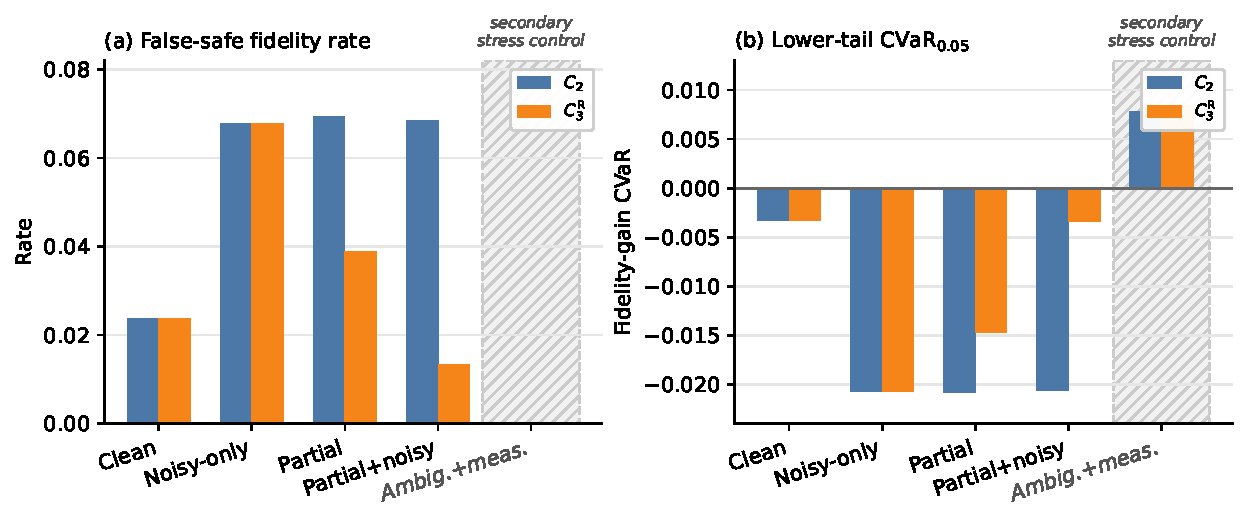
\includegraphics[width=0.95\textwidth]{c3r_downside_risk.pdf}
\caption{Historical submitted-grid downside-risk values for $C_2$ and
$C_3^{\mathrm R}$. Panel~(a) shows the false-safe fidelity rate $\mathrm{FS}_F$;
panel~(b) shows lower-tail fidelity gain $\mathrm{CVaR}_{0.05}$.  The patterns
are attributable to the submitted uncertainty gate and are not used as evidence
for a relational-spectral mechanism.}
\label{fig:c3r-downside-risk}
\end{figure}

The ambiguity-plus-measurement regime is informative for a different reason. Both
$C_2$ and $C_3^{\mathrm R}$ have zero false-safe fidelity rate in this regime, so
the binary false-safe metric alone would miss any distinction. The lower-tail
metrics and logical-success rate nevertheless improve slightly under
$C_3^{\mathrm R}$, indicating that false-safe rate should be interpreted together
with lower-tail and intervention diagnostics.

\subsection{Intervention quality: harmful blocks, missed gains, and net effect}
\label{subsec:results-intervention-quality}

The previous subsection records historical submitted-grid downside-risk values.
Because $C_3^{\mathrm R}$
can only veto proposed $C_2$ switches to $B$, the relevant quantities are
conditional on $C_2=B$.

In the partial-syndrome regime, $C_2$ selected $B$ in 1094 rows and
$C_3^{\mathrm R}$ blocked 476 of those switches, a conditional block rate of
0.4351. Among the blocked switches, the harmful-block precision was 0.8697: most
blocked switches were cases where staying with $A$ would have produced larger
fidelity gain than switching to $B$. The prevented loss was 12.2670, while the
missed beneficial gain was 6.6055, yielding a positive net intervention effect of
5.6616.

In the partial-plus-noisy regime, the intervention is stronger. $C_3^{\mathrm R}$
blocked 670 of 821 proposed $C_2$ switches to $B$, with harmful-block precision
0.8791 and harmful-switch recall 0.8475. The prevented loss was 17.4350 and the
missed gain was 8.3139, giving a net intervention effect of 9.1212. This shows
that the controller is not merely blocking more transitions. It blocks harmful
transitions with high precision, and the prevented harmful loss exceeds the missed
beneficial gain. The conditional intervention rates, aggregate balance, and 
normalized net effect across the active regimes are summarized in 
Fig.~\ref{fig:c3r-intervention-quality}.

\begin{figure}[t]
\centering
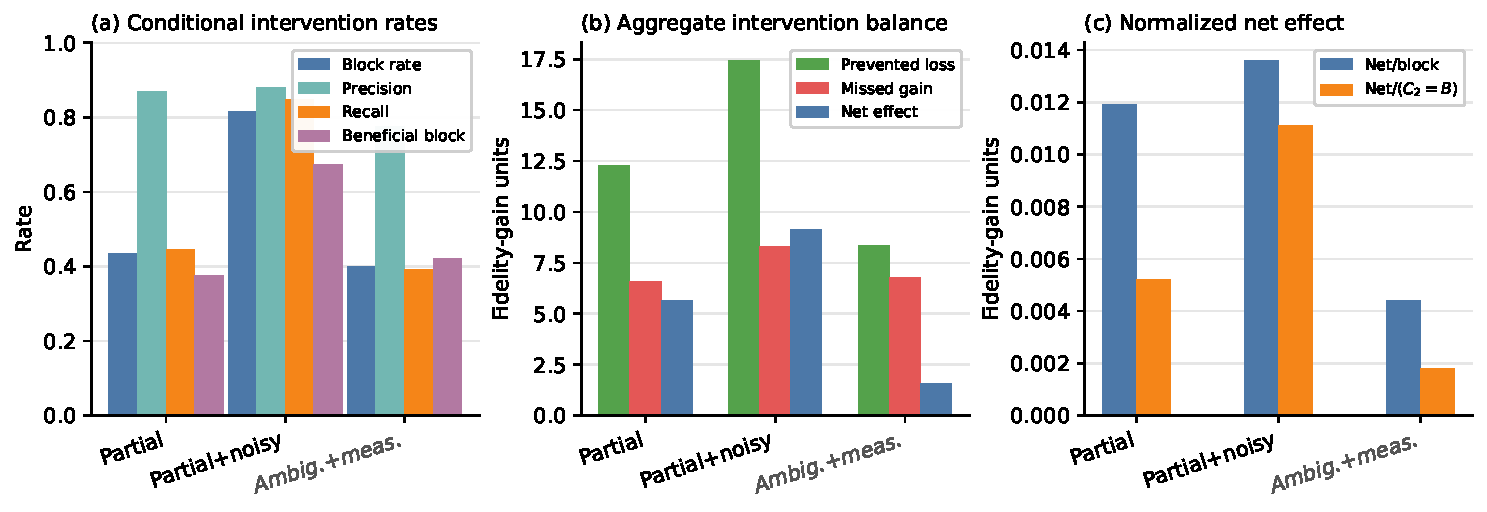
\includegraphics[width=0.95\textwidth]{c3r_intervention_quality.pdf}
\caption{Historical submitted-grid intervention diagnostics for $C_3^{\mathrm R}$
in regimes where it actively blocks $C_2$ switches. Panel~(a) reports the conditional intervention rates:
block rate (given $C_2=B$), harmful-block precision, harmful-switch recall, 
and beneficial-switch block rate. Panel~(b) shows the aggregate intervention 
balance, comparing prevented harmful-switch loss, missed beneficial-switch 
gain, and the resulting net effect, all in fidelity-gain units. Panel~(c) 
normalizes the net effect per blocked switch and per $C_2$-proposed switch 
to separate aggregate benefit from the number of vetoed proposals. The 
ambiguity-plus-measurement regime is hatched as a secondary stress control.}
\label{fig:c3r-intervention-quality}
\end{figure}

The cost of the controller is also visible. $C_3^{\mathrm R}$ blocks some
beneficial switches: the beneficial-switch block rate is 0.3750 in the partial
regime, 0.6739 in the partial-plus-noisy regime, and 0.4211 in the
ambiguity-plus-measurement regime. The observed benefit therefore should not be
described as free improvement. It is a risk-control tradeoff in which missed gains
are accepted only when the prevented losses are larger on the sampled grid.
The high beneficial-switch block rate in the partial-plus-noisy regime shows that
$C_3^{\mathrm R}$ is not an efficiency-maximizing selector. Its operating point is
intentionally conservative and should be evaluated by net downside-risk reduction,
including normalized net effect, rather than by switch acceptance alone.
This cost is substantial in the partial-plus-noisy regime, where more than half
of beneficial $C_2$ switches are also vetoed. The present operating point should
therefore be viewed as a safety-biased baseline rather than a tuned optimal
controller.

\subsection{Negative controls and observed operating limits}
\label{subsec:results-limitations}

The clean and noisy-only regimes serve as negative controls. In both cases,
$C_3^{\mathrm R}$ is effectively inactive and does not materially change the
$C_2$ outcomes. This is desirable: a risk-aware controller should not impose a
universal conservative bias when the syndrome evidence is either reliable or only
mildly corrupted without partial observability. The raw uncertainty mean is 0 in
the clean map and 0.038 in the noisy-only map, far below the saturation condition
that triggers uncertainty-based veto behavior.

The submitted partial-plus-noisy and partial rows have the largest
uncertainty-threshold effects. The ambiguity-plus-measurement regime provides a
weaker descriptive contrast: $C_3^{\mathrm R}$ changes logical-success rate from
0.5208 to 0.5978 and has positive net intervention value, while the binary
false-safe rate is already zero for both policies.  None of these submitted-grid
patterns identifies a relational-spectral mechanism or a decoder advantage.
Threshold diagnostics further show that setting $u_{\max}=1.00$ removes the veto
and recovers $C_2$ behavior, whereas stricter $u_{\max}=0.75$ increases blocking
and can reduce $\mathrm{FS}_F$ further at the cost of more beneficial-switch loss.
In some regimes this becomes overly conservative. Thus the default point is not
claimed to be optimal; it is a conservative operating point that exposes the
downside-risk tradeoff.

\section{Interpretation of the submitted-grid audit}\label{sec:discussion}

\subsection{What the submitted grid does and does not show}
\label{subsec:discussion-operating-zone}

The submitted rows establish only a descriptive operating pattern: the
uncertainty gate is inactive in clean and noisy-only rows and active in the
partial-observability rows.  They do not establish that relational spectral
evidence is useful, because the clock-conditioned densities are constant and
candidate $B$ is admissible in every row.  The audit separates this negative
finding from the new R3 held-out residual test below.

The strict-$C_3$ result is correspondingly non-informative: its condition does
not create an independent preferred zone, and the removed-uncertainty ablation
does not veto a single proposed switch.  We withdraw the former interpretation
of this observation as evidence for a more elaborate admissibility controller.

\subsection{Partial observability and decision geometry}
\label{subsec:discussion-partial-observability}

The submitted decision variables include a score difference, an admissibility
flag, normalized constraint violations, and an additive syndrome-stress index.
They are useful for reproducing the historical switch decisions, but their
geometry cannot be interpreted as a nondegenerate relational trajectory because
the conditional density is constant.

At the submitted default setting, the only empirically active conjunct is the
uncertainty saturation guard.  The policy is mathematically one-sided---it can
remove candidate-$B$ switches from the $C_2$ decision set but cannot create new
switches---yet this fact alone does not supply a physical or spectral mechanism.

The historical intervention metrics quantify the cost of that uncertainty-only
veto, including missed beneficial switches.  They are not used to claim a
mechanism or to optimize a gate across codes and noise models.

\subsection{Limits of the submitted recovery comparison}
\label{subsec:discussion-recovery-control}

The submitted candidate comparison is not a damaged-syndrome decoder benchmark.
Candidate $A$ used the complete circuit syndrome-recovery channel applied to the
underlying noisy density; damaged, missing, and ambiguous syndrome symbols
affected only the controller support.  Candidate $B$ is a discrete template
candidate, and its submitted admissibility flag never rejects a row.

The historical two-candidate values therefore do not answer a QEC recovery
question.  R3 replaces the information asymmetry with a count-record setting and
explicitly compares the template candidate to a continuous equal-information
estimate.  It retains false-safe rate as a selection-risk metric but does not
claim a decoder advantage.

The binary template-switching geometry remains a deliberately limited task.  It
makes conditional block and false-safe metrics computable, but a multi-candidate
or channel-level comparison requires a separate design.

\subsection{Clock-conditioned interpretation}
\label{subsec:discussion-background-independent}

The submitted Page--Wootters-type construction is not a valid finite relational
trajectory for the stated initial clock and Hamiltonians.  R1 supplies a valid
energy-matched finite-clock data construction, while R3 uses its clock labels as
split fitting and withheld validation records.  Neither construction is offered
as a foundations-level result about quantum time.

\subsection{Limitations and outlook}
\label{subsec:discussion-limitations}

The remaining limitations are substantive.  Larger codes, broader channel
families, optimized syndrome decoders, and multi-candidate recovery sets are
needed before making decoder-level claims
\cite{Asaka2026QuantumSpatialQEC,Filippov2024ScalabilityErrorMitigation,Li2025ZMixedAmplitudeDamping}.
R3 is a controlled two-candidate selection test, not a competitive QEC benchmark.

Alternative structural summaries, larger template banks, multipartite witnesses,
and learned representations may change the R3 switching sensitivity and need
independent tests~\cite{Brito2020MultipartiteInterference,Huang2026QuantumSpectralPDEs,Alexeev2025AIQuantumComputing}.

The current uncertainty variable is not a calibrated posterior.  In the submitted
grid it is the only observed active gate, while in R3 it is one of two fixed
calibrated switching thresholds.  Future work should calibrate uncertainty,
compare structural summaries, and test the task beyond the sampled finite-data
settings~\cite{Mohseni2021AdiabaticErrorSuppression,Lewis2026PulseQualityOptimisation}.

Taken together, the submitted-grid audit does \emph{not} support the previous
mechanistic attribution to relational spectral admissibility.  It establishes the
need for a physically specified finite-clock construction and an independent,
held-out gate ablation, which are provided next.

\section{Revision experiments and supported scope}\label{sec:revision-results}

\subsection{Physically specified finite-clock construction (R1)}

The revision experiments use an encoded logical qubit and an energy-matched
two-level clock, rather than the submitted $H_S=0$ setup.  Let
\begin{equation}
H_C=\omega Z_C,\qquad H_S=-\omega(n_xX_L+n_zZ_L),\qquad \omega=0.8,
\end{equation}
where the tilted setting is $n=(1,0,1)/\sqrt{2}$.  If $|n_+\rangle$ and
$|n_-\rangle$ are the logical eigenstates of $n_xX_L+n_zZ_L$ and
$|\psi\rangle=c_+|n_+\rangle+c_-|n_-\rangle$, we prepare
\begin{equation}
|\Psi\rangle=c_+|0\rangle_C|n_+\rangle_L+c_-|1\rangle_C|n_-\rangle_L,
\label{eq:revision-history-state}
\end{equation}
which obeys $(H_C+H_S)|\Psi\rangle=0$.  Eight clock effects
$E_k=(2/8)|\tau_k\rangle\langle\tau_k|$ at
$\tau_k=k\pi/(8\omega)$ form the finite POVM.  R1 verifies the null constraint,
conditional evolution, POVM completeness, nondegenerate clock geometry, and the
rank-three tilted observation design.  It is an observability qualification, not
a QEC efficacy result.

\subsection{Corrected held-out template-switching risk test (R3)}

R3 uses four frozen reference-bank, calibration, and held-out target stream
families.  Stream~0 reuses R2's random streams only to isolate the correction to
the gate definition; streams~1--3 use independent bank, calibration, target,
and measurement streams.  The controller receives finite-shot count records,
the known dynamics, and a fixed 32-state bank.  Four clock labels are fitting
labels and the complementary four are validation labels.  Candidate $A$ is a
continuous Bloch-ball projected weighted least-squares estimate and candidate
$B$ is the direct nearest template under the same fitting-label loss.

Let $L_{\mathrm{val}}(X)$ be the weighted squared loss of the unchanged
fitting-label candidate $X$ on the validation-label counts.  The held-out
residual statistic is
\begin{equation}
h=L_{\mathrm{val}}(B_{\mathrm{fit}})-L_{\mathrm{val}}(A_{\mathrm{fit}}).
\end{equation}
Neither candidate is refit on validation labels.  Score-only $C_2$,
uncertainty-only $U$, held-out-residual-only $H$, and the combined gate $C_3^R$
are evaluated on identical records.  Their three thresholds are fixed once from
the separate calibration set.  The target density is used only after a decision
to calculate fidelity.  An oracle nearest-template fidelity is reported only as
an offline bank-resolution diagnostic, never as a policy input.

In every one of the 24 grid cells in each of the four streams, $H-C_2$ has a
negative harmful-switch-rate difference whose two-way target-pair/measurement-
seed 95\% interval excludes zero.  At the fixed middle operating point
(bit-flip, 1,024 prepared copies, physical-noise probability 0.05, and readout
flip 0.05), the $H-C_2$ differences are $-14.844$, $-8.333$, $-10.677$, and
$-5.990$ percentage points in streams~0--3.  The $C_3^R-U$ difference is
negative in 12, 8, 12, and 6 cells, respectively; it is therefore not a uniform
increment over uncertainty-only selection.  The sign of the $C_3^R-A$ mean-
fidelity difference also varies across streams.  Full results and intervals are
reported in the Supplementary Information.

R3 consequently supports only a held-out residual safety filter for a discrete
template proposal.  It is not evidence for a spectral-representation advantage,
a uniform fidelity advantage over the continuous estimate, or a general
unknown-state QEC channel.

\section{Conclusion}\label{sec:conclusion}

We revised the paper after finding that the submitted clock construction was
degenerate and that its reported veto effect was not independently attributable
to admissibility.  Those findings are disclosed rather than repaired by changing
the interpretation of the submitted rows.  The revision supplies an explicit,
energy-matched finite-clock construction and a disjoint-calibration,
held-out-target switching experiment.

The revision supports a limited safety statement.  A corrected held-out residual
check can reduce the harmful-switch rate of a score-based discrete template
proposal.  Its combined uncertainty-plus-residual form does not have a uniform
increment over uncertainty-only selection, and it does not deliver a consistent
average-fidelity improvement over the continuous estimate.  We therefore do not
claim a decoder advantage, a spectral advantage over equal-information
estimation, or generic unknown-state recovery.

The contribution should therefore be read as a reproducible
negative-and-positive result: the submitted implementation does not validate the
originally proposed mechanism, while the replacement experiment validates a
narrower held-out residual filter under a specified finite-data
template-switching task.  The finite-clock construction is only a controlled data
construction, its uncertainty variable is not a calibrated posterior, and no
claim is made for larger codes, optimized decoders, multi-candidate recovery, or
generic unknown-state recovery.  Those questions require independently designed
experiments with full channel-level recovery metrics.

\funding{The authors received no specific funding for this work.}

\section*{Competing interests}
The authors declare no competing interests.

\data{The source code, simulation scripts, frozen protocols, and raw R3 outputs used in this study are available at \url{https://github.com/Jeong-Jaeyun/Risk-Aware-Relational-Spectral-Recovery-under-Partial-Quantum-Observability_Phase_1}. The archival submitted-grid materials are retained in the same repository.}

\roles{J.Y.J. conceived the study, implemented the simulations, performed the data analysis, and drafted the manuscript. H.Y.J. supervised the research, provided critical intellectual input, and revised the manuscript. All authors have read and approved the final version of the manuscript.}

\bibliographystyle{iopart-num}
\bibliography{reference}

\end{document}
